\documentclass{article}
\usepackage[utf8]{inputenc}
\usepackage{amsmath,amsfonts,amssymb,amsthm,mathtools}
\usepackage{parskip}
\usepackage{color}
\usepackage{booktabs}
\usepackage{hyperref}

\newtheorem{exercise}{Exercise}
\newtheorem{answer}{Answer}

\newcommand{\dd}[2][]{\frac{\partial #1}{\partial #2}}
\newcommand{\dt}[2][]{\frac{d #1}{d #2}}
\newcommand{\dL}{\dt[{\L}]}
\newcommand{\dLi}{\dt[{\Li}]}
\newcommand{\dLmb}{\dt[{\Lmb}]}
\newcommand{\dLfb}{\dt[{\Lfb}]}
\newcommand{\yh}{\hat{y}}

\newcommand{\bracket}[3]{\left#1 #3 \right#2}
\newcommand{\sqb}{\bracket{[}{]}}
\newcommand{\ab}{\bracket{\langle}{\rangle}}
\renewcommand{\b}{\bracket{(}{)}}
\newcommand{\abs}{\bracket{\lvert}{\rvert}}

\newcommand{\0}{\mathbf{0}}
\newcommand{\x}{\mathbf{x}}
\newcommand{\y}{\mathbf{y}}
\newcommand{\f}{\mathbf{f}}
\newcommand{\h}{\mathbf{h}}
\newcommand{\g}{\mathbf{g}}
\newcommand{\mom}{\mathbf{v}}
\newcommand{\F}{\mathbf{F}}
\newcommand{\gfb}{\g_\text{fb}}
\newcommand{\gmb}{\g_\text{mb}}
\newcommand{\gmbt}{\g_{\text{mb}; t}}
\newcommand{\gsmbt}{g_{\text{mb}; t}}
\newcommand{\gsfb}{g_\text{fb}}
\newcommand{\gsmb}{g_\text{mb}}
\newcommand{\gsd}{\g_\text{sd}}
\newcommand{\vh}{\hat{v}}
\newcommand{\gh}{\mathbf{\hat{g}}}
\newcommand{\gb}{\mathbf{\ab{g}}}
\newcommand{\gssqb}{\ab{g^2}}
\newcommand{\bv}{\mathbf{b}}
\newcommand{\ov}{\mathbf{o}}
\renewcommand{\a}{\mathbf{a}}
\newcommand{\X}{\mathbf{X}}
\newcommand{\W}{\mathbf{W}}
\newcommand{\I}{\mathbf{I}}
\renewcommand{\P}{\operatorname{P}\b}

\newcommand{\w}{\mathbf{w}}
\newcommand{\wo}{\w^*}

\renewcommand{\L}{\mathcal{L}}
\newcommand{\Li}{\L_i}
\newcommand{\Lmb}{\L_\text{mb}}
\newcommand{\Lfb}{\L_\text{fb}}
\newcommand{\E}{\operatorname{E}\sqb}
\newcommand{\Var}{\operatorname{Var}\sqb}

\newcommand{\logits}{\ell}
\newcommand{\vlogits}{\boldsymbol{\logits}}
\newcommand{\softmax}{\operatorname{softmax}}
\newcommand{\linear}{\operatorname{linear}}
\newcommand{\relu}{\operatorname{relu}}
\newcommand{\sqerr}{\operatorname{sqerr}}

\newcommand{\func}{\operatorname{func}}
\newcommand{\funcback}{\operatorname{func{.}backward}}
\newcommand{\funcjac}{\operatorname{func{.}jacobian}}
\newcommand{\inputs}{\operatorname{inputs}}
\newcommand{\outputs}{\operatorname{outputs}}

\newcommand{\linearback}{\operatorname{linear{.}backward}}
\newcommand{\reluback}{\operatorname{relu{.}backward}}
\newcommand{\sqerrback}{\operatorname{sqerr{.}backward}}

\newcommand{\linearjac}{\operatorname{linear{.}jacobian}}
\newcommand{\relujac}{\operatorname{relu{.}jacobian}}

\newcommand{\iinmb}{{i \text{ in mb}}}
\newcommand{\mbsize}{M}
\newcommand{\mbavg}{\tfrac{1}{\mbsize} \sum_{\mathclap{\iinmb}}}

\newcommand{\iinfb}{{i \text{ in fb}}}
\newcommand{\fbsize}{N}
\newcommand{\fbavg}{\tfrac{1}{\fbsize} \sum_{i=1}^{\fbsize}}
\newcommand{\lrtrad}{\eta_\text{trad}}
\newcommand{\lravg}{\eta_\text{avg}}

\title{EMAT31530, Part 6: Practical optimization in AI}
\author{Laurence Aitchison}
\date{}

\begin{document}

\maketitle

Now, we know how PyTorch computes gradients.
However, to optimize practical neural networks, you need a bit more than just gradients.
In this part, we'll see:
\begin{itemize}
  \item Minibatching.
  \item SGD with momentum.
  \item Preconditioning in general.
  \begin{itemize}
    \item RMSProp
    \item Adam
    \item AdamW
  \end{itemize}
  \item Other considerations:
  \begin{itemize}
    \item Local optima (their mysterious absence)
  \end{itemize}
\end{itemize}

\section{Minibatching}
So far, we've computed the full gradient based on all the training data in one big batch computation.
In deep learning, this is typically called a ``full batch'' method.
However, remember that GPU memory is very limited, and training datasets are often very, very large.
So full batch training only works in small-scale settings.

As an alternative, we usually use minibatches.
A minibatch is a small subset of the training data (e.g. 128 images out of 60,000 images in the full dataset).
In minibatched training, we calculate the loss, compute the gradients and update the parameters for only the minibatch.

To write down minibatched updates, we need notation for the gradient for an individual datapoint,
\begin{align}
  \g_i &= \dLi{\w}
\end{align}
where $\Li$ is the loss for an individual datapoint.
We can use the individual datapoint gradient to write down the minibatched gradient. 
The minibatched gradient is just the gradient, averaged over datapoints in the minibatch,
\begin{align}
  \gmb &= \mbavg \g_i =  \mbavg \dLi{\w}.
\end{align}
Here, $\mbsize$ is the minibatch size, and ``$\iinmb$'' gives the set of indicies of datapoints in the current minibatch.
However, it is quite awkward to use this expression directly in PyTorch, as, taken literally, it seems to involve backpropagating through $M$ single-datapoint losses, $\Li$.
In contrast, PyTorch only allows us to (easily) work with a single loss.
We therefore need to define a minibatched loss.
Note that we again use an \textit{average}, rather than a sum, as it makes the code + analytics slightly easier.
\begin{align}
  \Lmb &= \mbavg \L_i.
\end{align}
Using PyTorch to differentiate the minibatch loss gives 
\begin{align}
  \dLmb{\w} &= \dt{\w} \b{\mbavg \L_i} = \mbavg \dLi{\w} = \mbavg \g_i = \gmb,
\end{align}
which gives the required averaged gradients.

The simplest optimizer that uses minibatching is called ``stochastic gradient descent'', commonly abbreviated to SGD.
This is very similar to gradient descent that we've seen previously, but it uses minibatched gradients, rather than the full batch gradient,
\begin{align}
  \w_{t+1} &= \w_t - \eta \gmbt.
\end{align}
The ``stochastic'' in SGD refers to the stochasticity induced by randomness in the choice of minibatches.

This additional stochasticity raises a question: does SGD actually work?
Specifically, does it converge to the minimum of the loss?
Indeed, if you use a fixed learning rate, it will get close to the optimum, but won't actually exactly converge to exactly the optimum. 
Instead, it bounce around the optimum forever due to the ``noisy'' minibatched gradient estimates.

However, it turns out we can prove convergence in once setting: when the learning rate, $\eta$, goes to zero.
Specifically, we can show that if you reduce the learning rate $\eta$, and at the same time, consider an increasing number number of iterations, $T(\eta) = 1/\eta$, then you expect the SGD updates to move the parameters to the same place, but the variance decreasing variance, as we in-effect end up averaging over more samples of the minibatch noise.

To define the notion of the ``right expectation'', we need to go back to the original full batch setting.
Specifically, we're going to write the full batch loss again as an average,
\begin{align}
  \Lfb &= \fbavg \Li.
\end{align}
where $N$ is the number of datapoints in the full dataset.
The full batch gradient is again the average of individual datapoint gradients,
\begin{align}
  \gfb &= \dLfb{\w} = \fbavg \dLi{\w} = \fbavg \g_i.
\end{align}
Now, we can think of the indidivual datapoint gradient as a random variable, which is equally likely to be the gradient corresponding to any individual datapoint,
\begin{align}
  \P{\gsd} &= \fbavg \delta(\gsd - \g_i)
\end{align}
Critically, this random variable has the right expectation,
\begin{align}
  \E{\gsd} &= \fbavg \g_i = \gfb.
\end{align}
And as the minibatched gradient is just a bunch of independent realisations of $\gsd$, 
\begin{align}
  \E{\gmb} &= \gfb.
\end{align}
i.e.\ it also has the right expectation.

Thus, we interpreted the single-datapoint, $\gsd$, or minibatched, $\gmb$, gradients as random variables, and proved that they have the right expectation, $\gfb$.
In language from statistics, we could consider $\gsd$ and $\gmb$ as estimators of $\gfb$, and because the expectation is right, we say these estimators are ``unbiased''.
It turns out that having unbiased gradient estimates provably works: as the learning rate goes to zero, the noise in each minibatch estimate ``averages out'', and the method converges.
Specifically, as we reduce the learning rate, $\eta$, we consider an increasing number of timesteps,
\begin{align}
  \label{eq:T(eta)}  
  T(\eta) = \tfrac{1}{\eta}.
\end{align}
The overall change in the parameter, $w$ is,
\begin{align}
  \Delta w &= \eta \sum_{t=1}^{T(\eta)} \gsmbt.
\end{align}
Writing $\eta = 1/T(\eta)$,
\begin{align}
  \Delta w &= \frac{1}{T(\eta)} \sum_{t=1}^{T(\eta)} \gsmbt
\end{align}
Thus, $\Delta w$ is just the average of $T(\eta)$ independent realisations of the minibatched gradient, $\gsmbt$.
The expected change in weights is thus,
\begin{align}
  \E{\Delta w} &= \frac{1}{T(\eta)} \sum_{t=1}^{T(\eta)} \E{\gsmbt} = \frac{1}{T(\eta)} \sum_{t=1}^{T(\eta)} \gsfb = \gsfb,
\end{align}
which is just the full-batch gradient.
Moreover, as $\Delta w$ is the average of $T(\eta)$ independent realisations of the minibatch gradient, $\gsmbt$, the variance of $\Delta w$ is proportional to $1/T(\eta)$, or to $\eta$ (Eq.~\ref{eq:T(eta)}),
\begin{align}
  \Var{\Delta w} &= \tfrac{1}{T(\eta)} \Var{\gsmb(t)} = \eta \Var{\gsmb(t)},
\end{align}
Thus, as $\eta \rightarrow 0$, the variance in the change in weights $\Var{\Delta w}$ also goes to zero.
%
%such that the expected change in the parameter is the same,
%\begin{align}
%  \E{\Delta w} &= \E{\eta \sum_{t=1}^{T(\eta)} \gsmb(t)}\\
%  \intertext{As $\E{a (X + Y)} = a (\E{X} + \E{Y})$, where $X$ and $Y$ are random variables, and $a$ is a scalar,}
%  \E{\Delta w} &= \eta \sum_{t=1}^{T(\eta)} \E{\gsmb(t)}\\
%  \intertext{As $\E{\gsmb(t)} = \gsfb$ (and we assume that the full batch gradient doesn't change much over the short period we're considering,}
%  \E{\Delta w} &= \eta \sum_{t=1}^{T(\eta)} \gsfb
%  = \eta T(\eta) \gsfb
%  = \eta \tfrac{1}{\eta} \gsfb
%  = \gsfb.
%\end{align}
%Now, lets consider the variance.
%\begin{align}
%  \Var{\Delta w} &= \Var{\eta \sum_{t=1}^{T(\eta)} \gsmb(t)}\\
%  \intertext{As $\Var{a (X + Y)} = a^2 (\Var{X} + \Var{Y})$, where $X$ and $Y$ are independent random variables, and $a$ is a scalar,}
%  \Var{\Delta w} &= \eta^2 T(\eta) \Var{\gsmb(t)}
%  = \eta^2 \tfrac{1}{\eta} \Var{\gsmb(t)}
%  = \eta \Var{\gsmb(t)}.
%\end{align}
Hence, as $\eta \rightarrow 0$, the variance in the parameters also converges to zero, $\Var{\Delta w} \rightarrow 0$.

Theory is great, but deep learning is a practical subject, so there's a few points of ``wisdom'' and/or common practice. Specifically:
\begin{itemize}
  \item Each pass through the full training dataset is called an ``epoch''.  Deep learning training progress is typically measured in epochs.  Each epoch is composed of many minibatches (minibatches per epoch = dataset size / minibatch size).
  \item Within each epoch, it works slightly better to randomise the minibatches, rather than going through the same fixed set of minibatches at each epoch again and again (that's what \verb|shuffle=True| does).
\end{itemize}

\section{Momentum}

The simple form of SGD described above is rarely used in practice.
The problems all come down to the interactions between the size of gradients and the learning rates.
Specifically:
\begin{itemize}
  \item If all the gradients are small, then we'd like to use large learning rates to converge reasonably quickly.
  \item If all the gradients are large, then we'd like to use small learning rates to avoid instability.
\end{itemize}
The problem is in practice, gradients in some directions are large, and gradients in some directions are small.
In practice, that means you need to use a small learning rate (to avoid instabilities along directions with large gradients).
But that inevitably means you converge slowly in directions with small gradients.
Momentum is one way to mitigate these issues, as it allows you to push up the learning rate a bit, allowing faster convergence in the small-gradient directions, while avoiding instabilities in the large-gradient directions.
Specifically, the instabilities often look like the diagram below,
\begin{center}
  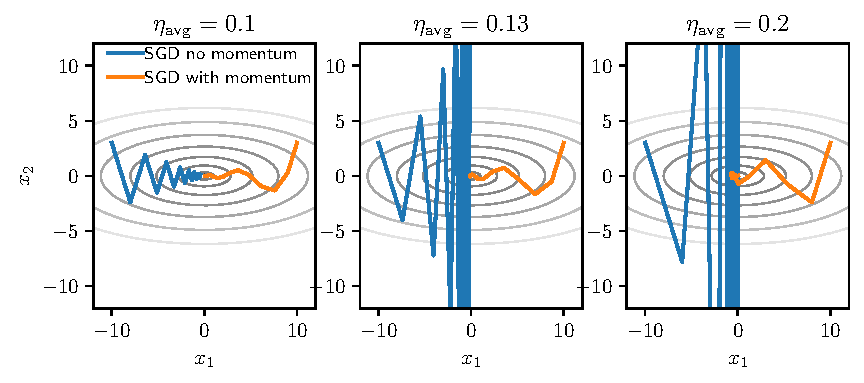
\includegraphics[width=\textwidth]{momentum.pdf}
\end{center}
If the learning rate is too large, SGD can jump over the optimum in that direction (in this case, we're looking at the large vertical jumps for SGD depicted in the blue line).
That's okay if you end up closer to the middle than you started (i.e.\ left plot below with $\eta=0.1$), in which case the gradient next time is smaller, and you will gradually converge on the right answer.
But if you end up further from the middle than you started (i.e.\ middle and left plots below), then you'll blow up.
Momentum (orange line) allows you to increase learning rates a bit while avoiding this instability.

How does momentum work?
One inuition for momentum (and the origin of the term ``momentum'') is the analogy with Physics.
Specifically, consider a ball rolling around on a hilly landscape, with friction. 
The objective, $\L(\w)$ describes the height of the landscape at any location, $\w$.
``Gravity'' pushes the ball downhill with a force given by the gradient
\begin{align}
  \F(\w) &= - \lrtrad \gfb.
\end{align}
Taking $m=1$, the equations of motion are,
\begin{subequations}
\begin{align}
  \dt[\mom]{t} &= - (1-\mu) \mom + \F(\w) = - (1-\mu) \mom - \lrtrad \gfb\\
  \dt[\w]{t} &= \mom.
\end{align}
\end{subequations}
Here, the $- (1-\mu) \mom$ term in the first equation represents friction ($\mu$ is between $0$ and $1$).
Discretising these equations with a timestep of $1$ and using the minibatched gradient, $\gmbt$ in place of the full batch gradient, $\gfb$, gives
%\begin{subequations}
%\begin{align}
%  \Delta \mom_t &= -(1-\mu) \mom_t - \lrtrad \gmbt\\
%  \Delta \w_t &= \mom_t
%\end{align}
%\end{subequations}
%which are the traditional momentum updates.
%Here, we use $\Delta \mom_t$ and $\Delta \w_t$ to mean the update in $\mom_t$ and $\w_t$ at this timestep,
%\begin{align}
%  \Delta \mom_t &= \mom_{t+1} - \mom_t & 
%  \Delta \w_t &= \w_{t+1} - \w_t.
%\end{align}
%Thus, the updates can also be written in a slightly simpler form,
\begin{subequations}
\begin{align}
  \label{eq:sgdm:trad:mom}
  \mom_{t+1} &= \mom_t + \dt[\mom]{t} = \mu \mom_t - \lrtrad \gmbt\\
  \label{eq:sgdm:trad:w}
  \w_{t+1} &= \w_t + \dt[\w]{t} = \w_{t} + \mom_{t+1}.
\end{align}
\end{subequations}
This is the parametrisation used in PyTorch (\href{https://pytorch.org/docs/stable/generated/torch.optim.SGD.html}{SGD docs}). Typically we use a momentum of $\mu=0.9$, while the learning rate, $\lrtrad$, needs extensive tuning.

However, I'm really not a fan of this parameterisation: it doesn't help us to understand what's really going on, and conflicts with how other learning rules such as Adam are written down.
These other learning rules use an exponential moving average gradient,
\begin{align}
  \label{eq:gb}
  \gb_{t+1} &= \beta_1 \gb_{t} + (1-\beta_1) \gmbt
\end{align}
This looks alot the ``velocity'' updates in Eq.~\eqref{eq:sgdm:trad:mom}, in that they both have an exponentially decay, with an additive term that depends on the minibatch gradient (the exponential decay is for $\mom$ in Eq.~\eqref{eq:sgdm:trad:mom} and for $\gb$ in Eq.~\eqref{eq:gb}).
However, the exponential moving average is much easier to interpret, as it is estimates the full batch gradient.
Specifically, if we are in a region where the underlying gradient doesn't change much,
\begin{align}
  \E{\gb_{t}} &= \gfb
\end{align}
(see exercises for details).
Now, we can write an alternative set of momentum updates,
\begin{subequations}
\begin{align}
  \label{eq:sgdm:avg:g}
  \gb_{t+1} &= \beta_1 \gb_t + (1-\beta_1) \gmbt\\
  \label{eq:sgdm:avg:w}
  \w_{t+1} &= \w_{t} - \lrtrad \gb_{t+1}
\end{align}
\end{subequations}
This is alot more similar to traditional SGD, in that the parameter updates are again just a learning rate times an estimate of the graident.
In SGD, we just use a single minibatched gradient estimate, while here, we use an exponential-moving-average over previous minibatch gradient estimates.
This averaging allows us to reduce alternating gradients (as in the original diagram), and stabilise learning at larger learning rates.

This raises a question: how does this ``average'' parameterisation relate to the ``traditional'' parameterisation?
It turns out that the ``velocity'' in the traditional formulation is just proportional to the exponential moving average gradient,
\begin{align}
  \mom_t &= - \frac{\lrtrad}{1-\mu} \gb_t.
\end{align}
To prove this assertion, we can substitute this into the traditional momentum updates (Eq.~\ref{eq:sgdm:trad:mom}),
\begin{align}
  \mom_{t+1} &= \mu \mom_t - \lrtrad \gmbt\\
  - \frac{\lrtrad}{1-\mu} \gb_{t+1} &= - \frac{\lrtrad}{1-\mu} \mu \gb_t - \lrtrad \gmbt
  \intertext{And dividing everything by $-\tfrac{\lrtrad}{1-\mu}$,}
  \gb_{t+1} &= \mu \gb_t + (1-\mu) \gmbt.
\end{align}
This is exactly the exponential moving average gradient in Eq.~\eqref{eq:sgdm:avg:g}, with $\beta_1 = \mu$.

Additionally, we can relate the learning rates in the two formulations.
Specifically, the traditional parameter updates (Eq.~\ref{eq:sgdm:trad:w}) are,
\begin{align}
  \w_{t+1} &= \w_{t} + \mom_{t+1} = \w_t - \frac{\lrtrad}{1-\mu} \gb_{t+1}.
\end{align}
This is equivalent to the average parameter updates (Eq.~\ref{eq:sgdm:avg:w}), if we set
\begin{align}
  \lravg = \frac{\lrtrad}{1-\mu}.
\end{align}
That means if we increase momentum (typically we use $\mu=0.9$) while keeping the traditional momentum, $\lrtrad$, the same, then we are in effect increasing the learning rate, $\lravg$.

\section{RMSProp}

If you remember, the original problem we were solving with momentum was that there are big gradients in some directions, and small gradients in other directions.
You ideally want a big learning rate in directions with a small gradient, to converge quickly.
At the same time, you want a small learning rate in directions with a big gradient, to avoid instability.
RMSProp gives you just that!
Specifically, RMSProp updates for a single parameter, $w$, are,
\begin{align}
  \gssqb_{t+1} &= \beta_2 \gssqb_{t} + (1-\beta_2) g_t^2\\
  \vh_{t+1} &= \frac{\gsmbt^2}{1-(\beta_2)^t}\\
  w_{t+1} &= w_t + \eta \frac{\gsmbt}{\sqrt{\vh_{t+1}} + \epsilon}
\end{align}
where $g_t$ is the minibatch gradient at iteration $t$.
You can understand this as being like SGD, but where 

so $\gssqb_{t+1}$ is an exponential moving average of the squared gradients, $g^2$.
Now, the update to the weights is always about $\eta$.
If we assume that we're in a small region, where the gradient is always the same, $g_t = \gsfb$, then, $\gssqb_{t+1} = \gsfb^2$, so the weight update is,
\begin{align}
  w_{t+1} &= w_t + \eta \frac{\gsfb}{\sqrt{\gsfb^2} + \epsilon} 
  \intertext{And $\sqrt{\gsfb^2} = \abs{\gsfb}$,}
  w_{t+1} &= w_t + \eta \frac{\gsfb}{\abs{\gsfb} + \epsilon}
  \intertext{For very small $\epsilon$,}
  w_{t+1} &= w_t + \eta \; \text{sign}(\gsfb) \\
  \text{sign}(x) &= \begin{cases}
     1 &\text{if } 0 < x\\
     0 &\text{if } 0 = x\\
    -1 &\text{if } 0 > x
  \end{cases}
\end{align}
So the magnitude of the updates is always around $\eta$, no matter how big the gradients are.

\section{Adam}

Adam is just RMSProp + Momentum.


\section{Appendix [Non examinable]}

\subsection{Exponential moving averages}
The exponential moving average gradient estimator was,
\begin{align}
  \gb_{t+1} &= \beta_1 \gb_t + (1-\beta_1) \g_t
\end{align}
But in what sense is this an ``exponential moving average''?

We know,
\begin{align}
  \gb_{t} &= \beta_1 \gb_{t-1} + (1-\beta_1) \g_{t-1}\\
  \gb_{t-1} &= \beta_1 \gb_{t-2} + (1-\beta_1) \g_{t-2}\\
  \gb_{t-2} &= \beta_1 \gb_{t-3} + (1-\beta_1) \g_{t-3}
\end{align}
Now, substituting $\gb_t$ into $\gb_{t+1}$,
\begin{align}
  \gb_{t+1} &= \beta_1 (\beta_1 \gb_{t-1} + (1-\beta_1) \g_{t-1}) + (1-\beta_1) \g_t\\
  \gb_{t+1} &= \beta_1^2 \gb_{t-1} + (1-\beta_1) (\g_t + \beta_1 \g_{t-1}).
\end{align}
Now, substituting $\gb_{t-1}$ into this expression,
\begin{align}
  \gb_{t+1} &= \beta_1^2 (\beta_1 \gb_{t-2} + (1-\beta_1) \g_{t-2}) + (1-\beta_1) (\g_t + \beta_1 \g_{t-1})\\
  \gb_{t+1} &= \beta_1^3 \gb_{t-2} + (1-\beta_1) (\g_t + \beta_1 \g_{t-1} + \beta^2 \g_{t-2}).
\end{align}
If we continued doing this, we'd get,
\begin{align}
  \gb_{t+1} &= \beta_1^{t+1} \gb_{1} + (1-\beta_1) \sum_{\tau=0}^{t-1}\beta_1^{\tau} \g_{t-\tau}
\end{align}
Additionally, we assume that we initialize $\gb_1 = \0$,
\begin{align}
  \gb_{t+1} &= (1-\beta_1) \sum_{\tau=0}^{t-1}\beta_1^{\tau} \g_{t-\tau}
\end{align}
This can be interpreted as a weighted average, 
\begin{align}
  \gb_{t+1} &= \sum_{\tau=0}^{t-1}w_\tau \g_{t-\tau}
\end{align}
with weights,
\begin{align}
  w_{\tau} &= (1-\beta_1) \beta_1^{\tau}
\end{align}
For this to be an exponential moving average, we need the sum of the weights to be $1$.
\begin{align}
  \sum_{\tau=0}^{t-1} w_{\tau} &= (1-\beta_1) \underbrace{\sum_{\tau=0}^{t-1} \beta_1^{\tau}}_{\mathclap{\text{geometric series}}}
\end{align}
For geometric series, we know,
\begin{align}
  \sum_{k=0}^{n-1} r^k &= \frac{1-r^n}{1-r}
\end{align}
(for $0 \leq r < 1$).
Therefore,
\begin{align}
  \sum_{\tau=0}^{t-1} w_{\tau} &= (1-\beta_1) \frac{1-\beta_1^t}{1-\beta_1} = 1-\beta_1^t
\end{align}
As $0 \leq \beta_1 < 1$, it will quickly approach $0$ as $t$ gets large. 
In that case, the sum of weights approaches $1$, and it makes sense to regard Eq.~\eqref{eq:gb} as an exponential weighted average.

\end{document}

